\begin{equation*}
    p\left(
    % with tikzpicture environment
    \underset{\mathllap{
    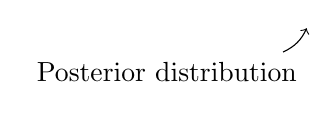
\begin{tikzpicture}
      \draw[->] (-0.3, 0) to[bend right=20] ++(0.3,2ex);
      \node[below left] at (0,0) {Posterior distribution};
    \end{tikzpicture}
  }}{$\theta$}
        |y \right) = \frac{p(y|\theta) \dot p(\theta)}{p(y)}
\end{equation*}


\begin{equation*}
  x
  % with tikzpicture environment
  \underset{\mathllap{
    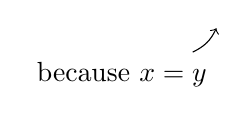
\begin{tikzpicture}
      \draw[->] (-0.3, 0) to[bend right=20] ++(0.3,2ex);
      \node[below left] at (0,0) {because $x = y$};
    \end{tikzpicture}
  }}{=}
  y + x - x
  % with tikz command
  \overset{\mathclap{\tikz \node {$\downarrow$} node [above=1ex] {trivial};}}{=}
  y + y - y
\end{equation*}

\tikzstyle{every picture}+=[remember picture]
\everymath{\displaystyle}

Using tikz:

\begin{equation*}
   p(\theta
   \tikz[baseline=-1pt]{
     \node (eq)
     {$\vert$};
   }
   y)
\end{equation*}


\begin{tikzpicture}[overlay]
   \node (t) at ($(eq) + (-0.5,-0.5)$) {\footnotesize Posterior Distribution};
   \path[->,shorten >= 6pt] (eq.base) edge [bend left=10] (t.mid) ;
\end{tikzpicture}


Using underset:

\begin{equation*}
   x \underset{\mathrm{def}}{=} y
\end{equation*}
